\documentclass[10pt,letterpaper]{article}

% ---- NeurIPS-like page layout (5.5in x 9in text block, Times 10pt) ----
\usepackage[letterpaper,left=1.5in,right=1.5in,top=1in,bottom=1in,
            textwidth=5.5in,textheight=9in,headheight=0pt,headsep=0pt,
            footskip=0.4in]{geometry}
\usepackage[T1]{fontenc}
\usepackage[utf8]{inputenc}
\usepackage{mathptmx}
\usepackage{microtype}
\usepackage{amsmath,amssymb}
\usepackage{graphicx}
\usepackage{booktabs}
\usepackage[font=small,labelfont=bf,skip=4pt]{caption}
\usepackage{titlesec}
\usepackage[hidelinks]{hyperref}
\usepackage{url}
\usepackage{xcolor}

\setlength{\parindent}{0pt}
\setlength{\parskip}{5.5pt}
\linespread{1.0}

\titleformat{\section}{\large\bfseries}{\thesection}{0.6em}{}
\titleformat{\subsection}{\normalsize\bfseries}{\thesubsection}{0.6em}{}
\titlespacing*{\section}{0pt}{12pt plus 2pt minus 2pt}{5pt}
\titlespacing*{\subsection}{0pt}{9pt plus 2pt minus 2pt}{3pt}

\renewcommand{\thefootnote}{\fnsymbol{footnote}}

% ---- Title block ----
\newcommand{\papertitle}{Delta Star: Space-Time A* Path Planning\\Among Moving Guards}

\begin{document}

\thispagestyle{empty}
\begin{center}
\rule{\textwidth}{4pt}\\[10pt]
{\Large\bfseries \papertitle}\\[8pt]
\rule{\textwidth}{1pt}

\vspace{14pt}
{\bfseries Shubham Patel}\\[2pt]
Dr. Bhimrao Ambedkar University\\
Agra\\
\texttt{shubhamkumarpatel45@gmail.com}
\end{center}

\vspace{10pt}
\begin{center}
{\large\bfseries Abstract}
\end{center}
\begin{list}{}{\setlength{\leftmargin}{0.5in}\setlength{\rightmargin}{0.5in}\setlength{\topsep}{0pt}}
\item
A robot on a grid has to reach a goal as fast as it can while guards walk on routes that are known in advance. A normal shortest path search looks only at walls, so it often walks into a guard. This paper describes Delta Star, a C++ planner that adds time to the state. Each state is a triple $(x, y, t)$, and waiting is one of the moves. The guard positions are put in a table before the search starts, so each move check takes constant time. The search is A* with the Manhattan distance as the estimate. On random $30 \times 30$ maps, a plain shortest path hit a guard in 16\,\% of the maps with 2 guards and in 76\,\% of the maps with 20 guards. Delta Star had no collisions in any map it solved. In the worst-case tests, a $100 \times 100$ grid with 1000 time steps and 20 guards needed about 9 million states, 1.75 seconds and 90 MB of memory.
\end{list}

\footnotetext{Preprint.}
\renewcommand{\thefootnote}{\arabic{footnote}}

% ======================================================================
\section{Introduction}

Path planning means finding a route from a start to a goal. Common methods such as breadth-first search, Dijkstra's algorithm \cite{dijkstra1959} and A* \cite{hart1968,wiki_astar} assume that the map does not change while the robot moves. This is not true when other things move on the map. A cell that is free now can be blocked one step later, and sometimes the best plan is just to wait.

This problem shows up in warehouses, where robots share aisles with forklifts and workers that follow a schedule. It also shows up in stealth games with patrolling guards, in drones or rovers that cross an area while scheduled vehicles pass through, and in contest puzzles.

Searching over position and time together is not new. It is often called Space-Time A*, and an early form of it is in the work of Erdmann and Lozano-P\'erez \cite{erdmann1987}, and a well-known description for the grid case is given by Silver \cite{silver2005}. This paper presents my own C++ version of that idea. It adds a fast move check, tests, benchmarks, and a separate brute-force checker. The code and a contest-style problem built on it are in the same repository.

The main points of this paper are:
\begin{itemize}\setlength{\itemsep}{0pt}\setlength{\topsep}{2pt}
\item a planner over $(x, y, t)$ where waiting is a normal move;
\item a table of guard positions that makes each move check $O(1)$;
\item measurements of time, states and memory in the worst case;
\item a comparison with a plain shortest path on random maps, counting collisions.
\end{itemize}

\section{Related work}

\textbf{Planning with time as a dimension.} Erdmann and Lozano-P\'erez \cite{erdmann1987} planned paths among moving objects by searching in a space made of position and time. Silver \cite{silver2005} used the same idea on a grid for many agents. In his Cooperative A*, each agent searches over $(x, y, \text{time})$ and avoids the routes that other agents have already reserved. He also gave two faster versions, Hierarchical Cooperative A* and Windowed Hierarchical Cooperative A*, which use a cheaper heuristic or limit how deep the search goes in time. Delta Star uses the same state, but for the simpler case of one robot and guards with fixed routes.

\textbf{Safe intervals.} Safe Interval Path Planning (SIPP) \cite{phillips2011} keeps one state for each safe time interval of a cell, and not one state for each time step. The authors show that it keeps the same optimality and completeness as planning with time as a dimension, and that it is much faster in tests with up to 200 moving obstacles. An anytime version \cite{narayanan2012} returns a first path quickly and improves it while time is left. SIPP-style methods should use fewer states than Delta Star when a cell is blocked only a few times. Delta Star keeps one state for every time step, which is easier to read and to check, but its cost grows with $T$. This paper does not compare the two, and I leave that for future work.

\textbf{Many robots.} For many robots, Conflict-Based Search \cite{sharon2015} finds paths that are complete and optimal. Delta Star plans for one robot only, so it is a much smaller problem.

\textbf{Search basics.} A* \cite{hart1968} uses an estimate that never goes above the true cost to find a best path. Delta Star uses it with the Manhattan distance. Dijkstra's algorithm \cite{dijkstra1959} and breadth-first search are the same idea without an estimate.

% ======================================================================
\section{Problem}

We have a grid with walls, a start cell $S$, a goal cell $G$, and $K$ guards. The position of guard $i$ at time $t$ is $g_i(t)$, and it is known for every $t \le T$.

We want the smallest $t$ and a list of cells $v_0 = S, v_1, \dots, v_t = G$. Each step is a move to a neighbouring cell (up, down, left, right) or a wait. The rules are:
\begin{itemize}\setlength{\itemsep}{0pt}\setlength{\topsep}{2pt}
\item no cell $v_s$ may hold a guard at time $s$;
\item the robot may not swap places with a guard;
\item walls cannot be entered.
\end{itemize}

\section{Method}

\textbf{State.} A state is $(x, y, t)$. Because time is part of the state, the same cell at two different times is two different states. This is what lets the robot wait.

\textbf{Moves.} From $(x, y, t)$ the robot can go up, down, left, right, or wait. Each move takes one time step and leads to a state with time $t + 1$.

\textbf{Move check.} A move is allowed if the next cell is not a wall, no guard is on it at time $t + 1$, and the robot is not swapping places with a guard.

\textbf{Guard table.} Before the search, the position of every guard at every time is worked out and stored. A move check then takes $O(1)$ time. My first version checked every guard on every move, which cost $O(K)$ per move.

\textbf{Estimate.} The estimate is the Manhattan distance to the goal (see taxicab geometry \cite{wiki_taxicab}). It never goes above the true remaining time, because each step moves at most one cell. So the first time the goal comes out of the priority queue, the time found is the smallest possible.

\section{Complexity}

Let $W \times H$ be the grid size, $T$ the number of time steps and $K$ the number of guards.

\begin{table}[!ht]
\centering
\caption{Time and memory of each part.}
\label{tab:complexity}
\begin{tabular}{lll}
\toprule
Part & Time & Memory \\
\midrule
Build the guard table & $O(T \times K)$ & $O(W \times H \times T)$ \\
Search (worst case) & $O(W H T \log(W H T))$ & $O(W H T)$ \\
One move check & $O(1)$ & -- \\
\bottomrule
\end{tabular}
\end{table}

If the start is in a corner, the robot can only be at cells with $x + y \le t$ at time $t$. At time $t$ there are $\binom{t+2}{2}$ such cells, so the number of states is at most
\begin{equation}
\sum_{t=0}^{T} \binom{t+2}{2} = \binom{T+3}{3}.
\end{equation}
For $T = N$ this grows like $N^3$.

\section{Experiments}

In the worst-case tests the goal was made unreachable. The search then cannot stop early and has to visit every state it can reach. All numbers below come from my own benchmark program. Times depend on the machine, so other computers will give different values.

\subsection{Time and states}

Table~\ref{tab:square} shows square grids with $T = N$. Every measured count is just below the bound $\binom{T+3}{3}$ from Equation~(1), which is 1\,771, 39\,711, 176\,851 and 302\,621 for these four rows. Figure~\ref{fig:bench}(a) plots time against $N$ on log axes, with a dashed line for $N^3$. The measured line follows the dashed line closely, except that the point at $N = 100$ lies a little above it.

\begin{table}[!ht]
\centering
\caption{Square grids with $T = N$ and an unreachable goal.}
\label{tab:square}
\begin{tabular}{rrrr}
\toprule
Grid $N \times N$ & $T$ & States expanded & Time \\
\midrule
$20 \times 20$ & 20 & 1\,746 & 0.2 ms \\
$60 \times 60$ & 60 & 39\,558 & 5.5 ms \\
$100 \times 100$ & 100 & 176\,493 & 39 ms \\
$120 \times 120$ & 120 & 301\,927 & 53 ms \\
\bottomrule
\end{tabular}
\end{table}

\begin{figure}[!ht]
\centering
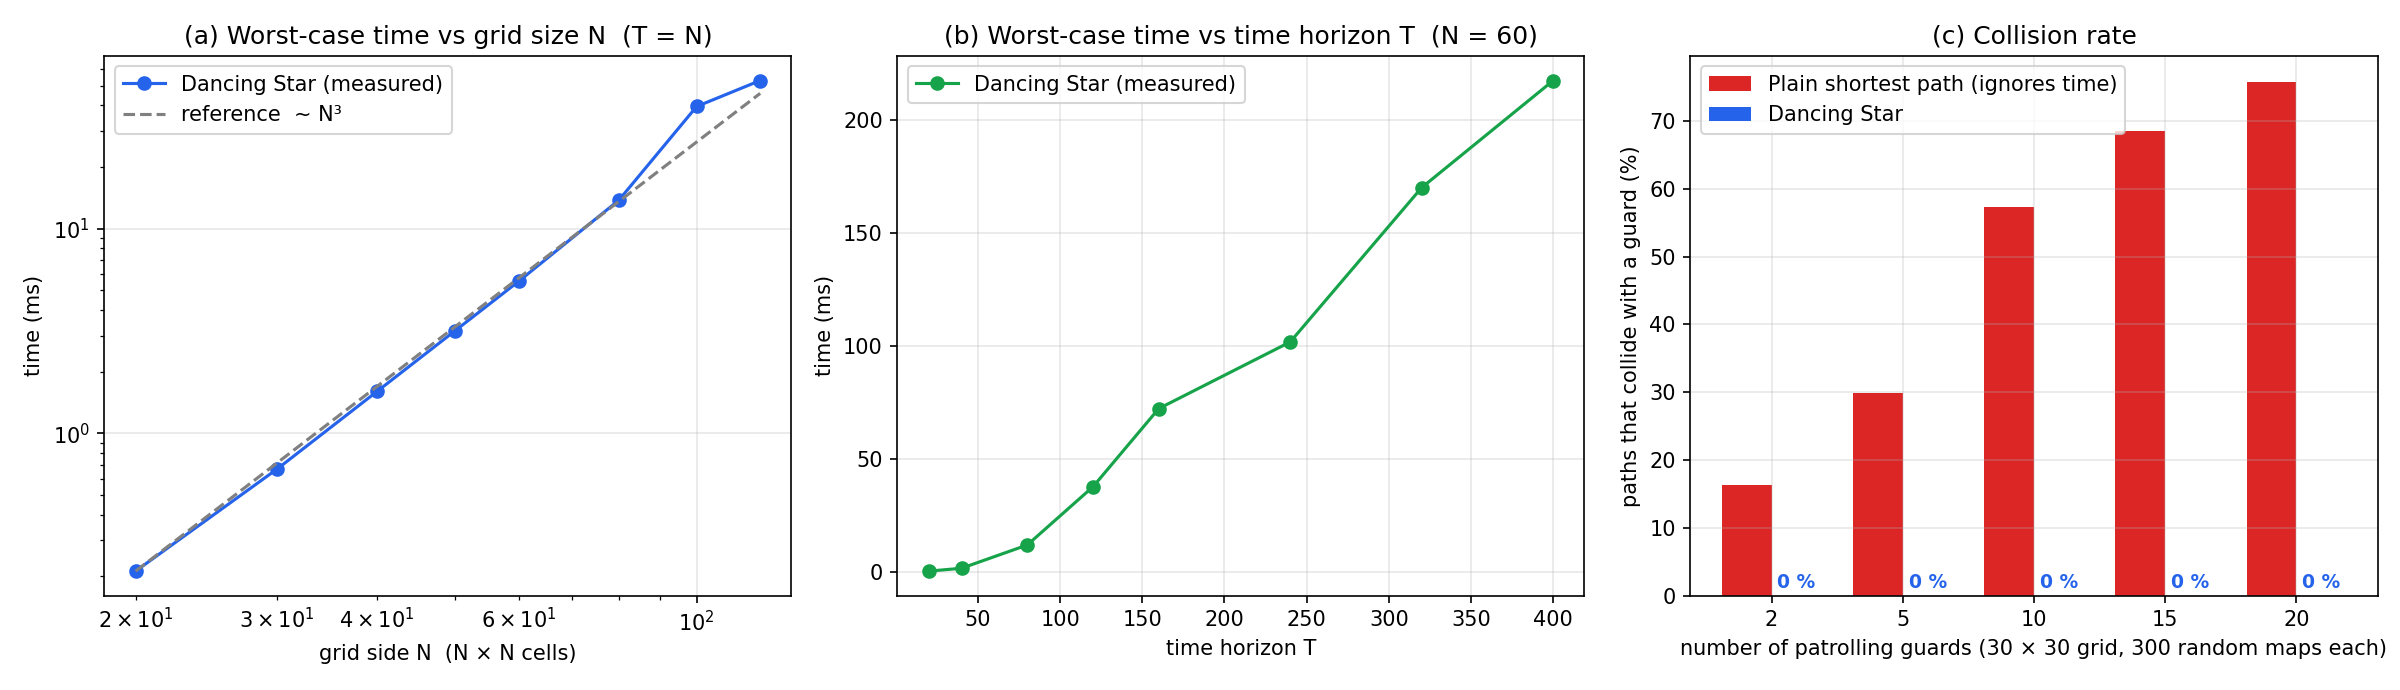
\includegraphics[width=\textwidth]{benchmark.png}
\caption{Benchmark results. (a) Worst-case time against grid size $N$ with $T = N$, on log axes; the dashed line is $N^3$. (b) Worst-case time against the time limit $T$ on a $60 \times 60$ grid. (c) Share of paths that collide with a guard on $30 \times 30$ random maps, 300 maps for each number of guards.}
\label{fig:bench}
\end{figure}

Figure~\ref{fig:bench}(b) keeps the grid fixed at $60 \times 60$ and changes $T$ from 20 to 400. The time grows with $T$ and reaches about 0.2 seconds at $T = 400$.

\subsection{Larger grids with 20 guards}

Table~\ref{tab:large} shows bigger runs. Going from $T = 500$ to $T = 1000$ on the $100 \times 100$ grid took the time from 0.81 s to 1.75 s. Memory follows about $9 \times W \times H \times (T + 1)$ bytes. For $100 \times 100$ and $T = 1000$ this is about 90 MB, the same as the measured value.

\begin{table}[!ht]
\centering
\caption{Worst cases with 20 guards and an unreachable goal.}
\label{tab:large}
\begin{tabular}{lrrrr}
\toprule
Grid & $T$ & States expanded & Time & Peak memory \\
\midrule
$50 \times 50$ & 200 & 375\,748 & 0.05 s & about 11 MB \\
$100 \times 100$ & 500 & 4\,009\,148 & 0.81 s & about 47 MB \\
$100 \times 100$ & 1000 & 8\,997\,648 & 1.75 s & about 90 MB \\
\bottomrule
\end{tabular}
\end{table}

\subsection{Collisions}

We compared Delta Star with a plain shortest path that looks only at walls and ignores time. Both ran on random $30 \times 30$ maps with 2, 5, 10, 15 and 20 guards, using 300 maps for each guard count (Figure~\ref{fig:bench}(c)). The plain shortest path hit a guard in 16\,\% of the maps with 2 guards and in 76\,\% of the maps with 20 guards. Reading the bars in the figure, the values for 5, 10 and 15 guards are about 30\,\%, 57\,\% and 68\,\%. Delta Star had 0 collisions at every guard count. It solved about 1\,380 of the 1\,399 maps. In the others, no safe path existed within the time limit.

\subsection{An example run}

Figure~\ref{fig:demo} shows one small map with walls and 2 guards. The robot goes from $S$ in the top left corner to $G$ in the bottom right corner in 16 steps. The Manhattan distance between $S$ and $G$ is $10 + 6 = 16$, so the robot did not lose any time.

\begin{figure}[!ht]
\centering
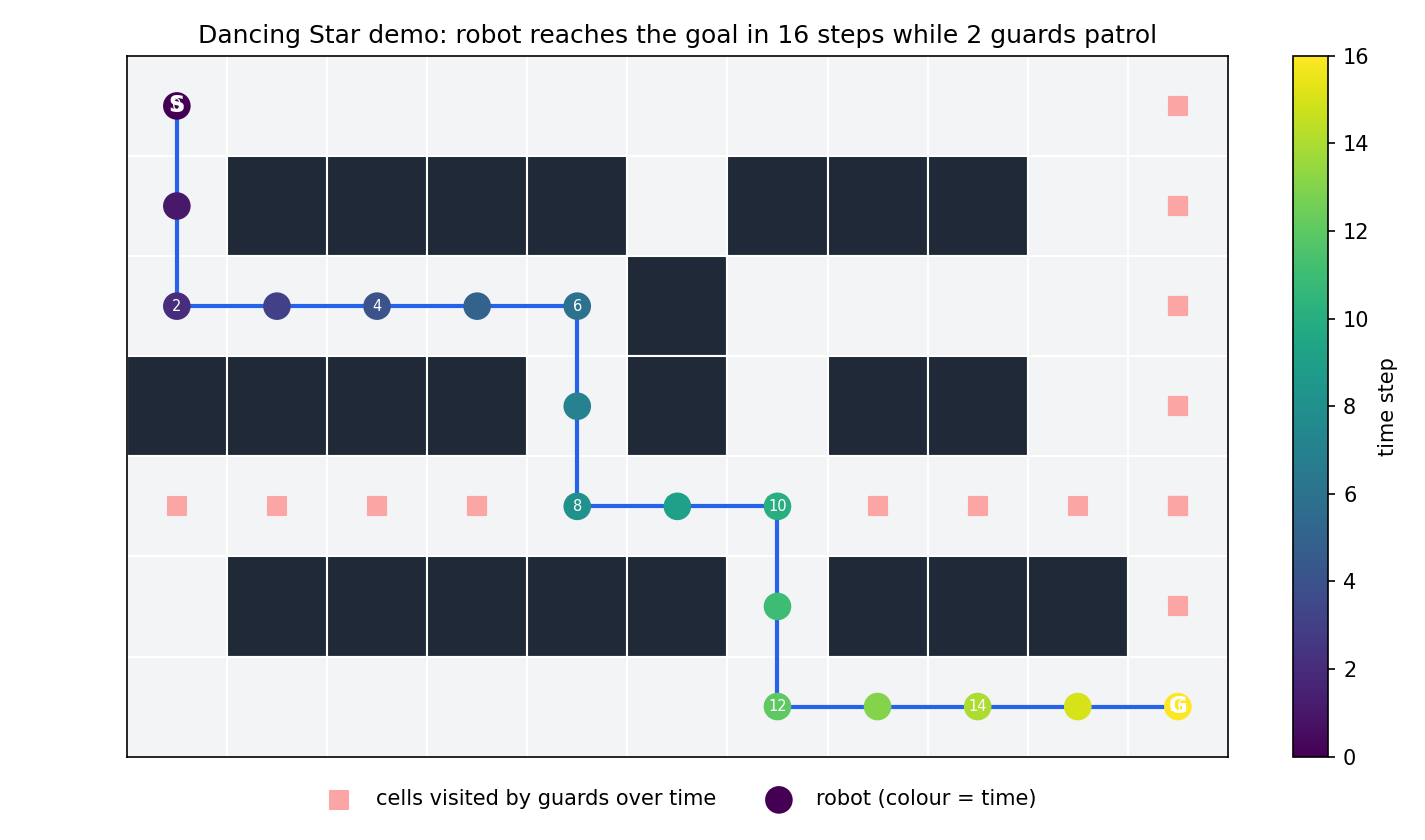
\includegraphics[width=0.85\textwidth]{demo_path.png}
\caption{A demo path. Dark cells are walls, pink squares are cells that guards visit over time, and the robot's colour shows the time step.}
\label{fig:demo}
\end{figure}

\subsection{Checking the answers}

A separate brute-force solver, written by me in Python, was run against the C++ code on 300 random small maps. The two never disagreed.

\section{Limits}

\begin{itemize}\setlength{\itemsep}{0pt}\setlength{\topsep}{2pt}
\item Time moves in whole steps. A move and a wait both cost 1.
\item Only four directions are allowed. Diagonal moves would break the Manhattan estimate.
\item Guard routes must be fixed and known. If guards move in ways we cannot predict, the planner has to run again every few steps.
\item Guards do not react to the robot. Two guards may stand on the same cell.
\item The start cell must be free at $t = 0$.
\item The code allows at most 32 guards, because it uses one bit per guard in a \texttt{uint32\_t}.
\item ``Not found'' means the goal cannot be reached within $T$ steps. It does not mean it can never be reached.
\item Memory grows with $W \times H \times T$, so long time limits on big grids need a lot of memory.
\end{itemize}

\section{Conclusion}

Adding time to the state lets A* handle guards that move on known routes, and it lets the robot wait when waiting is best. A table of guard positions makes each move check take constant time. In these tests the planner never hit a guard, while a plain shortest path hit one in up to 76\,\% of the maps. The price is time and memory that grow with the number of time steps.

Possible next steps are to compare Delta Star with SIPP on the same maps, to make waiting cost more, to add a penalty for cells next to a guard, to let guards move at random and plan again every few steps, and to plan for several robots together.

\section*{Code availability}

The code, tests, benchmarks and the contest-style problem are in the Delta Star repository (MIT license).

\begin{thebibliography}{12}\small
\setlength{\itemsep}{2pt}
\bibitem{hart1968} P.~E. Hart, N.~J. Nilsson, and B.~Raphael. A formal basis for the heuristic determination of minimum cost paths. \emph{IEEE Transactions on Systems Science and Cybernetics}, 4(2):100--107, 1968.
\bibitem{dijkstra1959} E.~W. Dijkstra. A note on two problems in connexion with graphs. \emph{Numerische Mathematik}, 1:269--271, 1959.
\bibitem{erdmann1987} M.~Erdmann and T.~Lozano-P\'erez. On multiple moving objects. \emph{Algorithmica}, 2:477--521, 1987.
\bibitem{silver2005} D.~Silver. Cooperative pathfinding. In \emph{Proceedings of the AAAI Conference on Artificial Intelligence and Interactive Digital Entertainment (AIIDE)}, 1(1):117--122, 2005.
\bibitem{phillips2011} M.~Phillips and M.~Likhachev. SIPP: Safe interval path planning for dynamic environments. In \emph{Proceedings of the IEEE International Conference on Robotics and Automation (ICRA)}, pages 5628--5635, 2011.
\bibitem{narayanan2012} V.~Narayanan, M.~Phillips, and M.~Likhachev. Anytime safe interval path planning for dynamic environments. In \emph{Proceedings of the IEEE/RSJ International Conference on Intelligent Robots and Systems (IROS)}, pages 4708--4715, 2012.
\bibitem{sharon2015} G.~Sharon, R.~Stern, A.~Felner, and N.~R. Sturtevant. Conflict-based search for optimal multi-agent pathfinding. \emph{Artificial Intelligence}, 219:40--66, 2015.
\bibitem{wiki_astar} Wikipedia contributors. A* search algorithm. \emph{Wikipedia, The Free Encyclopedia}. \url{https://en.wikipedia.org/wiki/A*_search_algorithm}
\bibitem{wiki_taxicab} Wikipedia contributors. Taxicab geometry. \emph{Wikipedia, The Free Encyclopedia}. \url{https://en.wikipedia.org/wiki/Taxicab_geometry}
\end{thebibliography}

\end{document}
